%!TEX root = ../masters.tex

\chapter{Introdução}
\label{cha:introduction}

\comment{Este texto inicial foi reformulado, corrigindo conjunções e aumentando a ligação entre as informações, já dando uma deixa para a apresentação do Contexto, que vem a seguir. Pequenas correções ortográficas foram feitas ao longo deste texto introdutório também.}

A necessidade de contribuição acontece de forma natural no ser humano. Os desejos em ajudar ao próximo e inclusive contribuir com alguma parte de sua formação é algo que desperta um desejo cada vez mais amplo do ponto de vista social.

Somos seres realizados pela satisfação do outro, e seu sucesso de uma forma ou outra acarreta em nosso sucesso, nossa satisfação pessoal e de certa forma também profissional. Sentimos atraídos por contribuir e por compartilhar conhecimento, sendo ele umas das principais formas de realização como pessoa.

Com o crescimento da pesquisa em todo o mundo um grande número de publicações foram inseridas no meio, fazendo com que uma infinidade de material estivesse disponível em poucos segundos. Deste modo, a necessidade de centralização automatizada dos dados e a contribuição dentre os pesquisadores é inerente ao desenvolvimento desta área. 

No âmbito acadêmico sempre contribuímos de uma forma ou outra com a formação de nossos colegas e parceiros de pesquisa. Esta contribuição pode ser feita com base em uma conversa informal ou até mesmo com uma ajuda em documentação ou sugestão de um texto para leitura. Esta sugestão de leitura geralmente possui um caráter muito técnico, e envolve na maioria dos casos a utilização de artigos acadêmicos, objeto central de análise e estudo deste trabalho.

\begin{textedited}
Sabemos da existência de bases de conhecimento nacionais e internacionais, porém, quando estamos falando da contribuição social, em pequena escala, interpessoal, estamos falando de contribuições físicas, com envio de sugestões de artigos para nossos amigos pesquisadores. Este envio é feito de maneira informal, reduz tempo e aumenta consequentemente a praticidade do processo de pesquisa.
\end{textedited}

Sendo assim, esta experiência como objetivo global seria uma ferramenta poderosa de apoio à pesquisa, com pesquisadores compartilhando conhecimentos de maneira informal, anônima, e segura. Esta forma de disseminação de conhecimento traria um benefício muito grande socialmente falando, uma vez que pesquisadores iriam se unir, mesmo que virtualmente, na transmissão de conhecimento, fazendo do processo da pesquisa um processo mais focado e desta maneira evitando o desperdício de tempo durante a fase de pesquisa em busca por conhecimento.

Para isso, a utilização de técnicas de extração de metadados deve ser utilizada de maneira eficaz, para que, de maneira automática, diversos artigos sejam analisados e catalogados em pequenos universos de pesquisa. Entende-se por metadados os campos básicos e necessários para que uma pesquisa por título de um artigo, por exemplo, seja feita com sucesso. Resume-se então que os metadados que esperam-se ser extraídos destes artigos são: o título do artigo, o nome e e-mail de seus autores, o resumo/\textit{abstract} e as referências utilizadas no texto.

Basicamente estes campos já permitem que uma pesquisa mais detalhada fosse feita e então o artigo localizado. Já as referências são necessárias para se fazer referências inversas de autores que publicam e são citados posteriormente, facilitando ainda mais aos pesquisadores poder, por exemplo, encontrar artigos semelhantes de uma mesma área do conhecimento.

\begin{figure}
	\centering
	\caption{Processo de Extração de Metadados}
	\label{fig:introduction}
	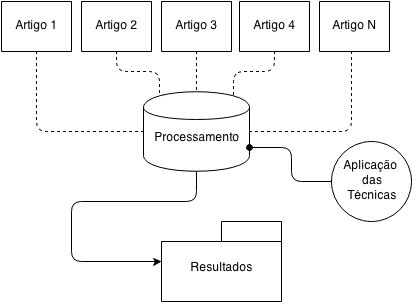
\includegraphics[width=0.7\linewidth]{./assets/images/introduction}
\end{figure}

\section{Contexto}
\label{sec:context}

\comment{Seção nova. Fala um pouco sobre de que maneira a ideia do trabalho surgiu. Peço que avaliem se este tópico não ficou muito pessoal. Tentei escrevê-lo o menos possível em primeira pessoa.}

\begin{textnew}

A ideia desta pesquisa surgiu de uma necessidade pessoal durante a disciplina de Fundamentos da Ciência da Informação. Era necessária a leitura de um artigo científico de um determinado autor, porém, este era muito difícil de se encontrar disponível na Internet, o que fez com que tivesse de recorrer ao professor da disciplina para consegui-lo.

Após o envio deste artigo pelo professor, conforme solicitado, surgiu a seguinte reflexão:

\begin{quote}
	\textit{''Esta contribuição ocorreu de maneira pessoal, entre mim e o professor, porém, se existisse um local onde os pesquisadores pudessem contribuir com o envio destes artigos este processo seria muito mais rápido e eficaz. Seria como se pudéssemos encontrar o artigo instantaneamente, dentro de nossa necessidade temporal. Seria pesquisador ajudando pesquisador.''}
\end{quote}

Desta forma, inclusive por minha formação acadêmica na área de Ciência da Computação, e por minha experiência profissional de mais de uma década em desenvolvimento Web, surgiu a ideia de desenvolver uma ferramenta de contribuição entre pesquisadores, totalmente online e independente. Todavia, estes repositórios de artigos já existiam na Internet e eram bem populados por sinal, porém, todos com um certo caráter comercial, com uma empresa ou instituição por trás, objetivando venda e lucro de uma maneira ou outra.

A ideia do desenvolvimento desta ferramenta ecoou durante dias, visto sua ampla aplicabilidade, como também sua contribuição social para com o universo da pesquisa, facilitando a vida de pesquisadores ao redor do mundo, sem complicações. Porém, para sua eficácia no armazenamento dos artigos enviados era necessária uma análise automatizada dos conteúdos destes arquivos, de maneira a extrair as partes mais importantes, como título, autores e referências, para que pudessem ser catalogados de maneira organizada e estruturada, a fim de facilitar a busca e permitir uma performance satisfatória por parte do usuário. Estes dados retirados dos documentos analisados são referenciados neste projeto pelo nome de ''metadados'', e são detalhados mais a frente de maneira aprofundada.

Sendo assim iniciou-se minha pesquisa pelo campo da extração de informação e principalmente pelo \textit{machine learning}, levando ao objeto central deste projeto, de maneira a identificar as características de cada ferramenta disponível atualmente e suas melhores aplicações dentro deste universo. Nada mais justo que contribuir com um projeto de pesquisa tendo como base fundamental o resultado de uma pesquisa acadêmica.

\end{textnew}

\section{Problema}
\label{sec:problem}

\comment{O problema foi reformulado, visando a identificação com o objetivo e resultados esperados.}

\begin{textnew}
Diversas ferramentas e técnicas para extração de metadados em artigos podem ser facilmente encontradas com uma rápida pesquisa pela Internet. Porém, algumas são propriedade de universidades ou até mesmo de instituições privadas, o que dificulta sua análise e teste, visto que seu código fonte é fechado, ou seja, sem acesso.
\end{textnew}

\begin{textedited}
As técnicas abordadas por este trabalho são aquelas cujo código fonte é aberto, ou seja, que pode ser analisado, testado e alterado, o que chamamos de projetos \textit{open source} (código livre).
\end{textedited}

De modo geral, estas técnicas livres de extração são focadas em \textit{layouts} (disposição visual) pré-definidos, geralmente seguindo modelos de conferências e/ou congressos internacionais, que possuem um padrão visual parecido, como é o caso do IEEE por exemplo, que serve de referência para diversos outros eventos da área da computação, tomando seu \textit{layout}, a princípio, como base.

Porém, existem diversos outros eventos que possuem \textit{layouts} de artigos considerados fora do padrão e, portanto, necessitam de adaptações destas técnicas para que seus trabalhos possam ser analisados e catalogados de maneira eficaz. Esta customização promoveria uma série de tentativas para verificar o melhor \textit{layout} para ser utilizado em cada caso, automaticamente.

\begin{textedited}
Algumas técnicas/ferramentas são aparentemente muito eficazes para um certo grupo de artigos, já seguindo um padrão visual pré-determinado. Porém, para alguns \textit{layouts} pouco comuns, de áreas do conhecimento diversas, espera-se que estas ferramentas não sejam tão eficazes, o que varia de acordo com a tecnologia aplicada e principalmente de acordo com o princípio teórico utilizado pelos seus autores, que será mais aprofundado nos próximos capítulos.
\end{textedited}

\section{Justificativa}
\label{sec:justification}

\comment{Justificativa foi reformulada.}

\begin{textedited}
Interessante notar a necessidade de centralização de artigos científicos para o meio acadêmico, além de permitir à contribuição coletiva, que seria uma forma de aumentar cada vez mais o acesso aos materiais de pesquisa. 

Diante disso, esta extração de metadados automatizada e eficaz traria benefícios para que estes repositórios de artigos fossem criados e catalogados com precisão\end{textedited}, tendo então milhões e milhões de documentos em suas bases de dados, prontos para serem pesquisados por pesquisadores de todas as nacionalidades e áreas do conhecimento.

\begin{textedited}
Este trabalho busca, portanto, identificar a melhor maneira que isso pode ser feito, levando em consideração o melhor resultado matemático possível dentro das técnicas e ferramentes disponíveis atualmente. Este resultado traria, para tanto, um ganho científico incalculável, permitindo que novas ferramentas e repositórios fossem criados e a disseminação do conhecimento fosse cada vez maior, e mais rápida.
\end{textedited}

\section{Histórico}
\label{sec:history}

\comment{Nova seção. Resolvi colocá-la, porém de maneira breve, para que sirva de uma introdução sobre o assunto e principalmente demonstrar a ligação da Ciência da Informação com a Ciência da Computação.}

\begin{textnew}

Os temas ''extração de informação'' e ''machine learning'' são resultantes da fusão de duas áreas do conhecimento bem complementares: a Ciência da Informação e a Ciência da Computação. Por esta proximidade, é muito comum encontrar artigos destes temas em ambas as áreas, porém com focos e objetivos diferentes.

Nesse sentido, essa união se complementa de maneira muito eficaz, visto a característica da fundamentação teórica da Ciência da Informação com a praticidade e desenvolvimento da Ciência da Computação. O resultado é um processo amplo e profundo, que permite que cada vez mais pesquisas sejam feitas e o ganho científico seja cada vez maior.

As pesquisas de \textit{machine learning} se iniciaram muito antes de se tornarem viáveis do ponto de vista tecnológico. Os primeiros registros desta pesquisa são datados de 1956 por \cite{machine-learning}, onde as primeiras teorias de aprendizado automatizado foram formuladas, utilizando-se para tal de conceitos matemáticos, defendendo a ideia do aprendizado por repetição e utilização de padrões.

Esta fundamentação ainda é muito utilizada e é a base para o desenvolvimento tecnológico existente na área de ''Inteligência Artificial''. Apesar de ser amplamente aplicada, os conceitos por trás desta fundamentação evoluíram ao longo das décadas, juntamente com a capacidade computacional, tornando os resultados muito mais reais e precisos do que era possível imaginar na formulação desta ideia.

Diante do cenário atual, com base no acelerado ritmo de desenvolvimento da tecnologia, bem como da evolução das técnicas de \textit{machine learning}, a utilização das ideias apresentadas décadas atrás ainda estão presentes e são amplamente utilizadas para o desenvolvimento de novas tecnologias e ferramentas.

Como é definido por \cite{foundations-machine-learning}, \textit{machine learning} atua como uma forma de aprendizado com base em experiências passadas, através da utilização de dados eletrônicos coletados que analisados posteriormente seguindo padrões definidos à máquina, de modo a permitir que ela possa fazer previsões com exatidão com base em sua experiência passada.

Este tema é muito amplo e sua aplicabilidade é extremamente ampla, permitindo a utilização de suas técnicas e teorias em diversas atividades, como classificação de textos e documentos, processamento de linguagem natural, reconhecimento de fala, detecção de fraudes, diagnósticos médicos e sistemas de recomendações, assim como mecanismos de buscas e extração de informação, ponto principal de discussão deste trabalho.

Dessa forma, este assunto tem sido discutido e pesquisado muito amplamente na Ciência da Informação, tanto nas áreas de classificação de documentos até mesmo em aplicações de buscas, unindo os conhecimentos adquiridos desta área do conhecimento com a evolução computacional presente nos dias atuais, onde a Ciência da Computação ganha força e nos permite realizar experimentos mais eficazes.

\end{textnew}

\section{Objetivos}
\label{sec:goals}

\comment{Os objetivos foram parcialmente reescritos, visando uma ligação maior com a metodologia, conforme observações feitas.}

\subsection{Objetivo Geral}
\label{ssec:main-goal}

Este trabalho possui como objetivo geral \begin{textedited}identificar quais são as melhores técnicas de extração de metadados em artigos científicos e suas melhores aplicações, com base em um conjunto de documentos pré-selecionados para testes, dos mais diversos padrões e de diversas áreas do conhecimento.

Com efeito, esta identificação permite que resultados sejam comparados e confrontados, permitindo decidir qual técnica é melhor utilizada para cada padrão visual, abrangendo um conjunto cada vez maior de dados e tendo resultados cada vez mais precisos.

\end{textedited}

%A necessidade de adequação é uma tendência natural de qualquer ramo de atividade, de maneira a promover possibilidades de ferramentas auto-suficientes capazes de suprir as necessidades de grupos específicos de pesquisas, de eventos ou conferências, que possui padrões de apresentação de artigos personalizados e que demandam de uma análise diferenciada para que possa ser indexada e então analisada por sistemas de informação.

\subsection{Objetivos Específicos}
\label{ssec:specific-goals}

\begin{textedited}

Com base na diferenciação dos \textit{layouts} de artigos científicos, este trabalho tem como objetivos específicos identificar também pontos em que as técnicas de extração de metadados necessitam de adaptações por parte de seus usuários e desenvolvedores, permitindo desta forma uma ampliação do universo de aplicação e garantindo assim uma cobertura mais abrangente dos artigos científicos analisados.

Acredita-se que os padrões de extração existentes no mercado são, de maneira geral, insuficientes para suprir todos os padrões de artigos existente, limitando a apenas uma pequena parcela destes, dentro de um \textit{layout} específico, o que acaba gerando um desconforto e uma perda de credibilidade destas técnicas existentes atualmente.

\end{textedited}

\section{Resultados Esperados}
\label{sec:expected-results}

\comment{Texto parcialmente alterado para prover uma maior identificação com o objetivo e o problema da pesquisa, de maneira a criar uma ligação entre eles.}

\begin{textedited}

As formas de extração de metadados em artigos científicos são geralmente baseadas em \textit{layouts}, ou seja, em pequenos pedaços onde certos dados devem ser extraídos. Porém em virtude da grande diversidade de materiais produzidos, dos mais diversos padrões visuais existentes, este \textit{layout} padrão - geralmente utilizado em artigos científicos - não se mostra eficiente na abrangência total das necessidades da comunidade científica mundial. 

\end{textedited}

Sobre este aspecto, espera-se que certos artigos científicos não tenham seus metadados analisados de maneira eficaz por todas as técnicas de extração analisadas, uma vez que \begin{textedited}adaptações no código seriam necessárias a fim de permitir que outros padrões visuais de artigos fossem também analisados, aplicando então um dos fundamentos do \textit{machine learning}, o aprendizado. 

\end{textedited}

\begin{textnew}

Por fim, espera-se que, com esta análise aprofundada das técnicas existentes, as mais eficazes na extração de metadados sejam identificadas e analisadas, elevando então o ganho científico neste tema de suma importância para o desenvolvimento tecnológico.

\end{textnew}

\section{Estrutura}
\label{sec:structure}

Esta pesquisa é estruturada iniciando com uma \begin{textedited} breve introdução sobre o tema; a apresentação do contexto da pesquisa, bem como sua origem e motivação; a definição do problema; a justificativa; o histórico do trabalho, demonstrando suas origens e fundamentos históricos; os objetivos gerais e específicos e, por fim, os resultados esperados.\end{textedited}

O segundo capítulo tem como base o referencial teórico feito através de uma RSL (Revisão Sistemática de Literatura), tendo como base \cite{Kitchenham}, que propõe um passo-a-passo para um revisão de literatura eficaz de modo a atingir os resultados desejáveis com a pesquisa.

No terceiro capítulo temos a metodologia para o desenvolvimento do trabalho, as técnicas que serão aplicadas e principalmente como serão feitas. \begin{textedited}Posteriormente, no capítulo quarto temos a análise e apresentação dos resultados, explicando como os testes foram realizados, os ambientes de teste criados e os resultados coletados.\end{textedited}

No quinto capítulo temos a discussão/conclusão, trabalhos futuros e considerações finais sobre o trabalho apresentado.


%\section{Limitações do Trabalho}
%
%Este trabalho limita-se aos artigos científicos difundidos na comunidade científica em formato PDF, excluindo aqueles em que seu conteúdo é disponibilizados através de imagens escaneadas de documentos físicos, o que impede, em um primeiro momento, de ter os textos analisados em sua forma original, sem necessidade de processamento extra a fim de obter todo o material textual contido em tais imagens. Além disso o trabalho pressupõe que a língua inglesa seja utilizada como padrão
%
%% Sobre os servidores com Windows
%
%Já na questão de testes de cada técnica de extração de metadados, as técnicas que serão selecionadas deverão ser de código livre/aberto, ou seja, ter seu uso liberado sem a necessidade de pagamento de licenças. Deste modo excluímos todas as técnicas que necessitam de \textit{softwares} proprietários para funcionar, por exigir licenças e fugirem das previsões de teste deste projeto. Assim, os projetos deverão necessariamente utilizar de linguagens de programação livres (ou de código aberto) e que rodem em sistemas operacionais derivados do Unix, como o Linux, por exemplo.

